% Chapter Template

\chapter{Network Design} % Main chapter title

\label{Chapter3} % Change X to a consecutive number; for referencing this chapter elsewhere, use \ref{ChapterX}

NVT Network follows two crucial principles in building an efficient product value prediction market:

\begin{itemize}
\item In a regular efficient market, there is not such thing as a free lunch. One has to pay to gain. In NVT Community, in order to incentivize users to discover good quality content, boosters and reviewers will be rewarded with NVT Tokens. This is a ”game” in which a return is expected, thus it has to come with an initial cost to balance the expected return. Therefore, each boost will cost a given amount of NVT Tokens, to prevent BOT cheating or manipulation.
\item It is imperative to treat every user with justice and fairness in order to build a free and truly decentralized market. Each user of the community will be able to get proportional rewards according to their contributions. The same way as a start-up company assigns its initial stocks to the employees with each major contribution. Every form of ”labor” should be valued equally and just. Contributing time to create, discover and distribute product reviews and data should be valued equally as if one is contributing money. In some ways one could even argue that time is more valuable than money. Based on the principle of fairness, we need a consistent mechanism to reward those who are doing quality work. High-quality content tends to inspire others and results in further creation of more high-quality reviews and articles. Therefore, when users spend NVT Tokens to upvote or boost a product, the community needs to assign a reasonable portion of NVT Tokens to the product creator in order to reward their contributions. Similarly, product discoverer and explorer (Booster) should also be rewarded for accurately finding the true value of a product or listing. The community implements a mechanism that redistributes NVT Tokens from late voters to early voters. In this way early stage voters have a higher expected return of NVT.
\end{itemize}

%----------------------------------------------------------------------------------------
%	SECTION 1
%----------------------------------------------------------------------------------------

\section{Proof of Network}

By introducing Proof of Network (PoN), the goal is to create an efficient, completely decentralized and community-driven prediction market. When users discover that the current score of a product is lower than their prediction or their expected valuation, they can boost or vote in order to positively alter the score of that particular product or network group. Every boost will cost a small amount of NVT Tokens or influence points.

This way, users that choose to participate and positively contribute to the community, have a higher chance to earn rewards more often, leading the users to actively try to discover worthy products, creators and deliver quality reviews.

%-----------------------------------
%	SUBSECTION 1
%-----------------------------------
\section{Product and Network Ranking}

NVT Community supports the creation of a community-driven and decentralized network value prediction market to make quality products stand out. Each stream or commit of information must be ranked based on the time that the post, the vote or the review was issued. The weight of each vote is calculated by taking the logarithm of total positive votes, adding it with the deposited NVT Tokens.

NVT Community users can enjoy additional rights by purchasing NVT Tokens and by locking them on the platform. Only locked NVT Tokens are added to the extra voting power. By reducing the liquidity of NVT Tokens with the locking function, the stakeholders’ interests are tied with the community. This way, the users are encouraged to implement judicious planning schemes, for their own self-interest.

Arbitrary votes would jeopardize the utility and community effect of the platform, therefore NVT Token stakeholders are more likely to make prudent judgment. Enhanced voting power for product, network and listings ranking is only fair for this occasion. Meanwhile, the logarithm operation prevents major stakeholders from having unchecked dictating powers. The voting weight for a popular post is inversely proportional to the rank of voters.

%-----------------------------------
%	SUBSECTION 2
%-----------------------------------

\section{Community Ecosystem}

NVT Community is composed of regular users, product creators, explorers and community moderators. Regular users can receive influence points by completing a given set of tasks. They can also be promoted to community ambassadors by contributing to the community. Users can be promoted to explorers by discovering quality products, networks and topics. They can also be elected as community moderators.

Explorers and content creators are considered core members in the development of the community. They will receive NVT Tokens as rewards for their contributed discoveries and posts. Network explorers can vote for topics and products in order to discover quality material for the community. Users can also vote for the highest performance contributing users so they can get extra NVT Tokens as rewards.

%----------------------------------------------------------------------------------------
%	SECTION 2
%----------------------------------------------------------------------------------------

\section{User Moderation}

Community moderators are elected every few weeks from regular users. The probability of a user being selected is proportional to the NVT Tokens one is staking on the platform. When someone gets elected as moderator by the community, it will result in NVT Token rewards. Community moderators ensure that the NVT Community is operating smoothly without problems and have some extra privileges when determining some future movements or decisions for the community.

One of the access levels of moderators, is the ability to delete questionable topics. To prevent abuse of such power, authors of removed content can appeal to the community. The appeal request would require a significant amount of NVT Token deposit. Users in the community can vote on the incident. Each vote would cost a small amount of NVT Tokens in order to prevent manipulation. After the appeal period has ended, if more than half of participants supports the notion, the appeal initiator would lose the deposit of NVT Tokens and the users who supported the appeal would also lose their NVT Tokens spent in the voting process. The same applies in the case of moderators losing the case vice-versa.

%----------------------------------------------------------------------------------------

\section{Community Rank}

The approach that is presented here is applicable to large scale decentralized databases which will be incorporated in the NVT Network. It can be implemented relatively straightforwardly, relying on observable data in comparison with input data from the community. This is of notable importance given that a product’s value is of interest not only to the retailer but also to external parties.

Intuitively, NVT Community Rank is based on a simple model of behavior: a consumer who ”browses” the community network randomly follows any one of the links on a page with equal probability. The algorithm is computed interactively and thus takes into account the effect of the entire network on each post, group or network. Mathematically, in each iteration, the algorithm divides a page’s Community Rank evenly among its successors (i.e., the pages it links to) in the network. Thus, the ranking of a page is ultimately the stationary probability that a random user who begins at a random page will visit the specific page.

Therefore, a page can gain a high community ranking by having either many pages or a few highly ranked pages that point to it. Although it is widely used as a measure of a node’s importance to a network, fundamentally, NVT Community Rank provides a proxy for the extent to which the network directs traffic to the node in question. NVT Rank can therefore be used as a benchmark value for the effect of the network on the traffic to a product’s page (and thus its demand).

%----------------------------------------------------------------------------------------

\section{Appeal System}

After the first appeal period ends, there is a cool-down timeframe in which if either the appeal initiator or the community moderator is unsatisfied by the result they can can start a second round of appeal. Next appeal will require exponentially more deposit than the previous one.

If the latest appeal is different from the previous one, the reward allocation for the previous one is voided and the final rewards are allocated based on the latest appeal result. This process is repeated until both party reach an agreement or either one is unwilling or unable to put down appeal deposit.

Community moderators will automatically assign a part of the NVT Tokens to users supporting them. If the appeal system overturns the original deletion, those NVT Tokens will be rewarded to users who disapproved of the deletion.

%----------------------------------------------------------------------------------------

\section{The Setting}

The revenue of a product is divided into two parts:

\begin{itemize}
\item The Intrinsic Value portion of the revenue is self generated by the item. It can be conceptualized as the revenue the product would be expected to yield on that website if it were not connected to others.
\item A product’s Incoming Value is driven by the recommendation links that point to that product from other products.
\end{itemize}

Thus, for product \textit{u}:

\begin{equation}
\textrm{Revenue(\textit{u})} = \textrm{IntrinsicValue(\textit{u})} + \textrm{IncomingValue(\textit{u})}
\end{equation}

We assume that an item’s Total Value consists of the product’s Intrinsic Value together with the product’s contribution to the Incoming Values of the products it recommends. The latter contribution is labeled as the ”Outgoing Value” of the focal product. We refer to the product’s total contribution to the firm (i.e., its Intrinsic Value together with its Outgoing Value) as its ”Network Value”:

\begin{equation}
\textrm{NetworkValue(\textit{u})} = \textrm{IntrinsicValue(\textit{u})} + \textrm{OutgoingValue(\textit{u})}
\end{equation}

This view is consistent with previous work assessing the value of customers in a network by distinguishing customers’ Intrinsic Value and the value they provide to the network.

%----------------------------------------------------------------------------------------

\section{PageRank as a Benchmark}

The goal of NVT Network is to develop an approach that will reallocate the value a product generates. It is suggested that this reallocation will be implemented according to the full recommendation system of the community group that the product is a part of.

Probably the best known computational tool that allows for a full network approach is PageRank, which is essentially an eigenvector centrality measure. This measure has been used for various applications involving ranking web pages. The best known application is Google’s ranking system, but PageRank has also been used for various academic research purposes, e.g. for understanding optimal advertising on the web.

The original PageRank algorithm provides a ranking of the importance of a web page in the hyperlinked structure of the web based on the following model:

\begin{equation}
\textrm{PageRank(\textit{u})} = \sum_{v \epsilon \textrm{ln(\textit{u})}} \frac{\textrm{PageRank(\textit{v})}}{\textrm{Out(\textit{v})}}
\end{equation}

where ln(\textit{u}) is the set of web pages (nodes) linking to node \textit{u} and Out(\textit{v}) is the number of outgoing links from node \textit{v}.

%----------------------------------------------------------------------------------------

\section{A Product Network Value Model}

The approach that is used to determine the network value of a product is similar to PageRank, with a fundamental difference. In sharp contrast with the existing methodology which considers only the traffic (value) that a product receives, in this work the traffic a product creates for other products is also considered.

Furthermore, similar to PageRank, different links (recommendations) generate different levels of traffic; thus, it is not enough to simply evaluate numbers of links. For example, in the context of Amazon, a link from Dan Brown’s best seller The Da Vinci Code is likely to be a more fruitful recommendation compared with one from a lower selling book.

The variable Impressions(\textit{v}) is defined as the number of people visiting product \textit{v}’s page (also frequently referred to as ”page views”) and observe its outgoing links. It is evident that not every link exposure leads to a purchase. Therefore, the recommendation conversion rate (RCR) associated with the product dyad (\textit{v},\textit{u}) is defined. RCR represents the probability that exposure to a link on \textit{v}’s page will result in a purchase of \textit{u}.

This probability is a combination of the probability that a link will be clicked on (frequently referred to as ”click through rate”) and the probability that the user’s visit to the next page will result in a purchase. Essentially, the RCR can be thought of as a ”cross selling conversion rate”.

We therefore define \textit{$a_{v \rightarrow u}$} an as the recommendation conversion rate (RCR) associated with the product dyad (\textit{v},\textit{u}); this RCR represents the probability that exposure to a link on \textit{v}’s page will result in a purchase of u. This probability is a combination of the probability that a link will be clicked on (frequently referred to as ”click through rate”) and the probability that the user’s visit to the next page will result in a purchase. Essentially, the RCR can be thought of as a ”cross selling conversion rate.

We can now define the Incoming Value of a product, that is, the sales that are attributed back to other products in the network, as:

\begin{equation}
\textrm{IncomingValue(\textit{u})} = \sum_{v \epsilon \textrm{ln(\textit{u})}} a_{v \rightarrow u} \times \textrm{Impressions(\textit{v})} \times P(u)
\end{equation}
where \textit{P(u)} is the price of product \textit{u}.

Note that the greater the volume of traffic directed to the product from neighboring products (i.e., the greater the number of Impressions of its neighbors or the links RCR), the larger the fraction of the product’s revenue that stems from its Incoming Value rather than its Intrinsic Value. For example, the Incoming Value of a book on Amazon that is recommended by many best sellers should be greater than that of a book that earns similar revenue despite not getting many recommendations or receiving recommendations from books that are not purchased often.

The remaining revenue generated by an item is by definition its Intrinsic Value (i.e., the revenue portion that is not generated by incoming links from other items in the network):

% \begin{equation}
% \textrm{IntrinsicValue(\textit{u})} = \textrm{Revenue(\textit{u})} - \textrm{IncomingValue(\textit{u})} = P(u) [ Q(u) - \sum_{v \epsilon \textrm{ln(\textit{u})}} a_{v \rightarrow u} \times \textrm{Impressions(\textit{v})}]
% \end{equation}

\begin{multline}
\textrm{IntrinsicValue(\textit{u})} = \textrm{Revenue(\textit{u})} - \textrm{IncomingValue(\textit{u})} \\ = P(u) [ Q(u) - \sum_{v \epsilon \textrm{ln(\textit{u})}} a_{v \rightarrow u} \times \textrm{Impressions(\textit{v})}]
\end{multline}

The outgoing value of item u is then the sum of all revenues that item u generates by recommending other products:

\begin{equation}
\textrm{OutgoingValue(\textit{u})} = \sum_{v \epsilon \textrm{Out(\textit{u})}} a_{u \rightarrow w} \times \textrm{Impressions(\textit{u})} \times P(w)
\end{equation}
where Out(\textit{u}) is the set of community group pages (nodes) to which node \textit{u} links.

Adding the Intrinsic Value of item \textit{u} to the product’s Outgoing Value, we obtain an expression for u’s Network Value:

% \begin{equation}
% \textrm{NetworkValue(\textit{u})} = \textrm{IntrinsicValue(\textit{u})} - \textrm{OutgoingValue(\textit{u})} = P(u) [ Q(u) - \sum_{v \epsilon \textrm{ln(\textit{u})}} a_{v \rightarrow u} \times \textrm{Impressions(\textit{v})}] + \sum_{v \epsilon \textrm{Out(\textit{u})}} a_{u \rightarrow w} \times \textrm{Impressions(\textit{u})} \times P(u)
% \end{equation

\begin{multline}
\textrm{NetworkValue(\textit{u})} = \textrm{IntrinsicValue(\textit{u})} - \textrm{OutgoingValue(\textit{u})} \\ = P(u) [ Q(u) - \sum_{v \epsilon \textrm{ln(\textit{u})}} a_{v \rightarrow u} \times \textrm{Impressions(\textit{v})}] \\ + \sum_{v \epsilon \textrm{Out(\textit{u})}} a_{u \rightarrow w} \times \textrm{Impressions(\textit{u})} \times P(u)
\end{multline}

where each product \textit{v} points to product \textit{u} and contributes to its incoming value, and product \textit{u}’s Outgoing Value stems from each product \textit{w} to which \textit{u} points. Note that a product cannot recommend itself and thus, by definition \textit{u} is unequal to \textit{v}.

% Figure 1: Sample Graph Containing Three Products
\begin{figure}[h]
\centering
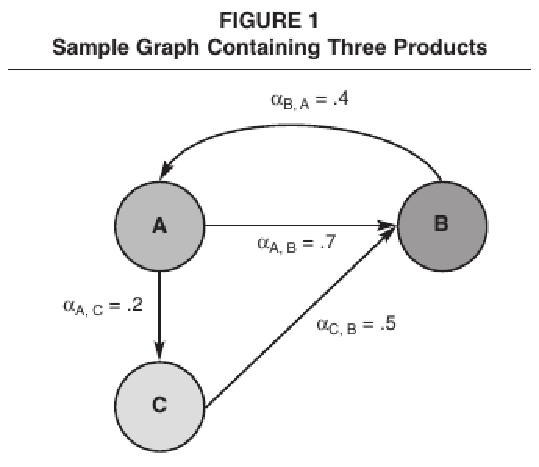
\includegraphics[]{Figures/figure_1}
\end{figure}

%----------------------------------------------------------------------------------------

\section{Quantifying Product Value}

A simple example is used to illustrate the application of the model. The definitions of the terms used are shown in Table 1. In Fig. 1, three linked products in an online e-commerce site are presented. RCRs and \textit{$a_{v \rightarrow u}$} are given and represent the probability that exposure to a link on \textit{v} will result in a purchase of \textit{u}.

Table 2 provides additional information on this small product network. For each Item (Column 1), the table presents the Quantity sold (Column 2), the Price per unit (Column 5), and consequently the total Revenue (Column 6).

The quantity of purchases of a product indicates the number of Impressions it receives (and thus recommendation exposure). However, Impressions can also stem from people who look at the product but do not purchase it. To move from Quantity

\begin{table}[ht]
\centering
\caption{Definitions}
\scalebox{0.45}{
\begin{tabular}{ll}
\hline\hline
\textbf{Term} & \textbf{Definition} \\ [0.5ex]
\hline
In(\textit{u}) & The set of web pages (nodes) linking to node \textit{u}. \\
Out(\textit{v}) & The set of web pages (nodes) to which node \textit{v} links. \\
P(\textit{u}) & The price of product \textit{u}. \\
Demand(\textit{u}) & The number of units of product \textit{u} sold. \\
Revenue(\textit{u}) & The total revenue a book generates (price x units). \\
Impressions(\textit{v}) & The number of people visiting product \textit{v}'s page (also frequently referred to as page views). \\
\textit{$a_{v \rightarrow u}$} & The PCR associated with the dyad (\textit{v,u}), which represents the probability that a customer exposed to a link to product \textit{u} on \textit{v}'s page will purchase product \textit{u}. \\
IntrinsicValue(\textit{u}) & The portion of product \textit{u}'s revenue that is not generated by incoming links from other items in the network. \\
IncomingValue(\textit{u}) & The sales of product \textit{u} that have been attributed back to the network. \\
OutgoingValue(\textit{u}) & The contribution of product \textit{u} to the incoming values of the product it recommends. \\
NetworkValue(\textit{u}) & The augmented value generated by a product that is part of a network. The sum of the product's intrinsic value and the value it generates for its neighbors through its outgoing links. \\
\textit{$k_u$} & The percentage of eventual buyers who viewed book \textit{u} and purchased book \textit{u}. \\
\hline
\end{tabular}}
\label{table:definitions}
\end{table}

\begin{table}[ht]
\caption{Network Value Algorithm Example, Iteration 1}
\centering
\scalebox{0.49}{
\begin{tabular}{c c c c c c c c c c}
\textbf{Item} & \textbf{Quantity} & \textbf{Impressions} & \textbf{Classical Conversion Rate} & \textbf{Price (\$)} & \textbf{Revenue (\$)} & \textbf{Intrinsic Value (\$)} & \textbf{Incoming Value (\$)} & \textbf{Outgoing Value (\$)} & \textbf{Network Value (\$)} \\
\hline
A & 10 & 13.33 & .75 & 100 & 1,000.00 & 975.00 & 25.00 & 145.33 & 1,120.33 \\
B & 5 & 6.25 & .80 & 150 & 750.00 & 395.71 & 354.29 & 25.00 & 420.71 \\
C & 20 & 28.57 & .70 & 20 & 400.00 & 394.67 & 5.33 & 214.29 & 608.95 \\
Total & & & & & 2,150.00 & 1,765.38 & 384.62 & 384.62 & 2,150.00 \\
\hline
\end{tabular}}
\label{table:example}
\end{table}

to Impressions, we can use a variable that is often reported for different e-commerce web sites, called the Conversion Rate. Conversion Rate is the percentage of page visits that actually result in a purchase (to differentiate this number from the cross product RCR, we label it the ”Classical Conversion Rate”). Thus, to get to the number of Impressions (Column 3), we can divide the Quantity (Column 2) by the Classical Conversion Rate (Column 4).

To understand the full value of each product, we first compute the Intrinsic and Incoming Values of each product. These refer, respectively, to the portion of the revenue that is self generated by the item (Intrinsic) and the portion of the revenue driven by the recommendation links pointing from other items to the focal item (Incoming). These values are presented in Columns 6 and 7 of Table 2.

Using Eq. 5, the Incoming Value of product B is computed:

% \begin{equation}

% \end{equation}

\begin{multline}
\textrm{IncomingValue(\textit{B})} = \sum_{v \epsilon \textrm{ln(\textit{B})}} a_{v \rightarrow B} \times \textrm{Impressions(\textit{v})} \times P(B) \\ = .07 \times 13.33 \times \$150 + .05 \times 28.57 \times \$150 \\ = \$139.96 + \$214.28 = \$354.29
\end{multline}

Using Eq. 6, the Intrinsic Value of product B is computed:

\begin{equation}
\textrm{IntrinsicValue(\textit{B})} = \textrm{Revenue(\textit{B})} - \textrm{IncomingValue(\textit{B})} = \$750 - \$354.29 = \$395.71
\end{equation}

Note that product C is responsible for most of its own revenue (i.e., it has a high Intrinsic Value), whereas product B ”owes” almost half of its revenue to network traffic (i.e., it has a high Incoming Value).

The second step of our approach assigns the Incoming Value of each product back to its incoming links. For example, product B’s Incoming Value is \$354.29, which is assigned back to products A and C, in proportion to the strength of their recommendations. This results in \$139.97 being assigned to product A and \$214.28 being assigned to product C. Similarly, product A’s Incoming Value (\$25) is assigned back to B (its only incoming link), and product C’s Incoming Value (\$5.33) is assigned back to A (its only incoming link).

After assigning the Incoming Values back to the incoming links, we can compute the Outgoing Value of each product using Eq.(7). A product’s Outgoing Value is the sum of the Incoming Values that the focal product generates for its neighbors. Column 9 of Table 2 presents the Outgoing Value of each product. In our example, B was assigned product A’s Incoming Value, such that:

\begin{equation}
\textrm{OutgoingValue(\textit{B})} = \sum_{w \epsilon \textrm{Out(\textit{B})}} a_{B \rightarrow w} \times \textrm{Impressions(\textit{B})} \times P(w) = .04 \times 6.25 \times \$100 = \$25
\end{equation}

The last step is computing the Network Value of each product as the sum of its Intrinsic Value and its Outgoing Value, using Eq. 8. Column 10 of Table 2 presents the Network Value of each product. Note that the total Network Value over the entire network is equal to the total revenue. That is, our model simply redistributes the revenues among the products.

For product B the Network Value is:

\begin{equation}
\textrm{NetworkValue(\textit{B})} = \textrm{IntrinsicValue(\textit{B})} + \textrm{OutgoingValue(\textit{B})} = \$395.71 + \$25 = \$420.71
\end{equation}

Note that product C generates almost all its own revenues, and only 1.3\% of its revenues are generated by the community recommendation made by product A. Product B, in contrast, is very dependent on external recommendations, which generate 47.2\% of its revenue. After attributing the revenues back to the items that generated them, we observe that the revenue that product C generates by recommending other items is higher than 41\% of the revenue it generates through its own sales. Finally, note that the total Network Value of product C is much higher than its revenue.


%----------------------------------------------------------------------------------------

\section{Iterations and Convergence}

A fundamental question when exploring influence in networks is that of the ”ripple” effect: To what extent can we assume that the network value created by an item spreads in a contagion like way into the network, beyond the first degree of separation?

Take, for example, a product network in which item A recommends item B, which recommends item C, which recommends item D. Consider item B in that network. When applied once, the model attributes to item B a proportion of the revenue from sales of item C, and item A is attributed a proportion of the revenue from sales of item B. This assumes that the recommendation effect of an item stops at the books it recommends and no ripple effect process occurs.

However, the picture may be more complicated if there is some effect beyond the first degree of separation. Some of the revenue from sales of item C that is attributed to item B should actually be attributed backward to item A, which generated part of item B’s traffic to begin with. Indeed, B’s actual contribution to C’s revenue should be decreased by the proportion of A’s contribution to B. In the same manner, B has some part in C’s contribution to D’s revenue, in that some of C’s value comes from the incoming value driven by B. In other words, an item is entitled to a share of another item’s network value, not just its revenue.

It is important to note here that although theoretically we could envision effects that stretch deep inside the product network, we assume a strong decay across degrees of separation. This is consistent with findings from the community and social network literature that show that influence is locally bound, with some researchers suggesting three degrees of separation as the typical limit. It is also in line with findings that suggest that the average shopping basket on sites such as Amazon and Barnes \& Noble contains fewer than three items.

Consistent with previous research, influence decays across the network exponentially. With our approach, almost all the effect is confined to the decentralized community driven review network, and only a relatively small part travels through to higher degrees of separation.


%----------------------------------------------------------------------------------------

\section{Product Determinations}

Companies increasingly aim to optimize their product and brand portfolios by considering the value that each product generates and eliminating items that do not provide enough value. Given the possible discrepancy demonstrated between revenue and network value, firms should look beyond revenue when making such decisions. Note that this direction is similar to the transition in the customer management literature from viewing a customer’s value (and consequently the customer portfolio) as based solely on his or her purchases, to a broader view that also takes into account the customer’s effect on others through word of mouth.

% \begin{figure}[h]
%     \centering
%     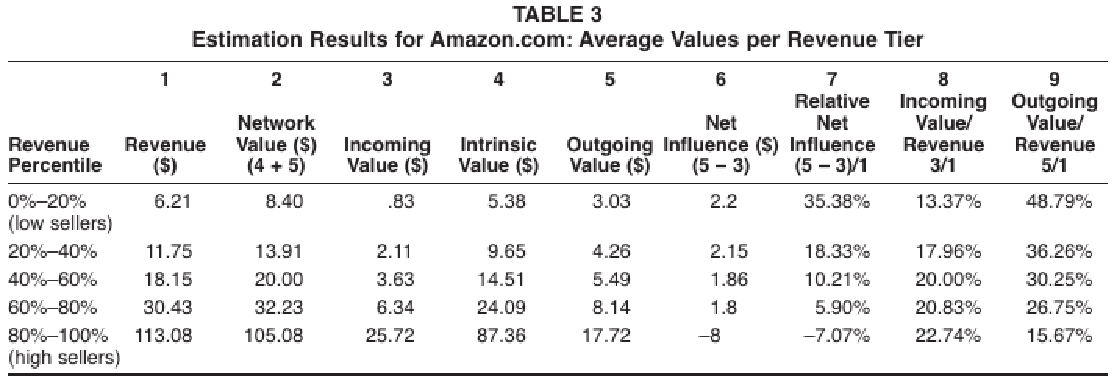
\includegraphics[width=\textwidth]{Figures/table_3.pdf}
% \end{figure}

The measure of the value to the firm created as a result of customers’ connectivity in the social network has been labeled customer referral value or customer social value. It should become of essential managerial importance as customers become more connected through tools such as social media and as marketers’ ability to follow

\begin{table}[ht]
\caption{Estimation Results for Amazon.com: Average Values per Revenue Tier}
\centering
\scalebox{0.32}{
\begin{tabular}{c c c c c c c c c c}
\textbf{Revenue Percentile} & \textbf{Revenue (\$)} & \textbf{Network Value (\$) (4+5)} & \textbf{Incoming Value (\$)} & \textbf{Intrinsic Value (\$)} & \textbf{Outgoing Value (\$)} & \textbf{Net Influence (\$) (5-3)} & \textbf{Relative Net Influence (5-3)/1} & \textbf{Incoming Value / Revenue 3/1} & \textbf{Outgoing Value / Revenue 5/1} \\
\hline
0\% - 20\% (low sellers) & 6.21 & 8.40 & .83 & 5.38 & 3.03 & 2.2 & 35.38\% & 13.37\% & 48.79\% \\
20\% - 40\% & 11.75 & 13.91 & 2.11 & 9.65 & 4.26 & 2.15 & 18.33\% & 17.96\% & 36.26\% \\
40\% - 60\% & 18.15 & 20.00 & 3.63 & 14.51 & 5.49 & 1.86 & 10.21\% & 20.00\% & 30.25\% \\
60\% - 80\% & 30.43 & 32.23 & 6.34 & 24.09 & 8.14 & 1.80 & 5.90\% & 20.83\% & 26.75\% \\
80\% - 100\% (high sellers) & 113.08 & 105.08 & 25.72 & 87.36 & 17.72 & -8 & -7.07\% & 22.74\% & 15.67\% \\
\hline
\end{tabular}}
\label{table:estimation}
\end{table}

this connectivity increases. Likewise, the ubiquity of decentralized product networks can make the network value of a product an important measure to help managers make informed product management decisions.

%----------------------------------------------------------------------------------------

\section{Product Network Influencers}

It is worthwhile to compare the results obtained regarding the ow of value in product networks with those obtained in research on social networks. Numerous studies have been devoted to the role of influencers and, in particular, hubs in social networks.

Who (or rather, which products) may be labeled ”influencers” in a product network? In most product networks, the number of outgoing links is limited, so a straightforward comparison to social network hubs is not trivial. More essential to the effect on others is the amount of traffic an item can send through its existing links, which we capture here in the number of impressions on the item’s page.

To connect influence to revenue tiers, we define influencers as the top 10\% in terms of outgoing value. The overall picture that emerges for the Amazon data is that the distribution of influence in the Amazon product network is spread across revenue tiers. Although the majority (56\%) of influencers are among the best sellers (top 20\% of revenue), the effect is still spread across other revenue tiers.

Another issue is that of net influence. Here, the comparison to social networks is limited, given that the research on the contribution of influencers in social networks has focused largely on the role of outgoing links, not incoming ones. If the influencers are defined as the group of products with the top 10\% of net influence, the best sellers are again most likely to be influencers. However in this case, they make up a smaller portion of the group (42\%), compared with influencers defined on the basis of outgoing value.

This result is particularly intriguing given that, on average, the net influence of this group is negative (see Table 3). Thus, it seems that there may be large differences among best sellers in terms of net influence, which are driven by incoming value.

%----------------------------------------------------------------------------------------

\section{Architectural Innovation and Performance Linkage}

Architectural innovation is described as an innovation that changed the way in which components of a product are linked together, while leaving the core design concept untouched. The core design concept explains the basic knowledge underlying the components. It destroys the usefulness of a firm’s architectural knowledge but preserves the usefulness of its knowledge about the product’s components.

In this description there is a distinction between the products as a whole (the entire system) and products in parts (components). The product as a whole explains how the components will work together. The components are defined as a distinct portion of the product that embodies a core design concept and performs a well defined function.

An example of an architectural innovation is the room air fan. The major components include the blade, the motor, the control system and the mechanical housing. The established technology is that of, large electrically powered fans, mounted in the ceiling. The introduction of a portable fan would be an architectural innovation. The primary components are largely the same, but the architecture of the product is quite different. There are also significant changes in the interactions between the components. For example the portable fan has a smaller size which means that there are new interactions between the motor size and the blade dimensions.

An architectural innovation draws attention to innovations that use many existing core design concepts in a new architecture and that therefore have a more significant impact on the relationships between components than on the technologies of the components themselves. The essence is to link existing components in a new way. The components themselves are not untouched. The central point is that the core design concept behind each component and the associated scientific and engineering knowledge remain the same. An architectural innovation is often triggered by a change in the components.

In the case of the room air fan the size is changed, that creates new interactions and linkages with other components in the established product. But it remains important that the core design concept behind the components stays the same.

%----------------------------------------------------------------------------------------

\section{Network Innovation}

A successful innovation depends on the spread of information and the exchange and combination of resources. Consequently the focus of innovation is found to be in networks and relations rather than in individual firms alone. Organizations build architectural knowledge around their relationships. Therefore communication channels, information filters and problem solving strategies play a significant role in architectural innovations.

An effective organization will organize itself around the product’s primary components in the network. These are the key relationships around which the organization builds architectural knowledge. An architectural innovation’s effect depends in a direct way on the nature of organizational learning about changes in architecture and about new interactions across components. The components are the key subtasks of the organization’s design problem.

%----------------------------------------------------------------------------------------

\section{Organizing Innovation}

How should the network be organized in order to improve the performance of an architectural innovation? It is argued that architectural innovation requires tight coordination across organizational boundaries. However it is unclear whether centralized, tight coordination by the innovation network’s leader improves architectural innovation. Next part will elaborate on the different influences of the level of betweenness on the innovation performance.

%----------------------------------------------------------------------------------------

\section{Network Decentralization}

The advantages and disadvantages of the level of betweenness within a network are elaborated. When should the lead firm organize innovation by using decentralized network approaches and when by using centralized network approaches? Centralized networks are those in which suppliers are tied to a ’lead’ firm. In decentralized networks suppliers have to meet the demands of diverse suppliers and customers by a market process or negotiation. Nobody in the network has total control.

The level of betweenness indicates the information control, it measures the centrality of a focal firm in a network and the extent to which a firm falls between pairs of other firms on the communication paths that link them. Betweenness is, in some sense, a measure of the influence a lead firm has over the information through the alliance network. The information control can be measured by the amount of network flow which is controlled by this firm.

Centralized or decentralized positions of a lead firm have different implications for innovations. The challenge for the lead firm is to choose the organizational form that matches the type of innovation they are pursuing the best. Why is a high level of betweenness (bureaucracy) bad, and a low level of betweenness (flexibility) good? Chesbrough and Teece (1996) argue that decentralized structures will be more responsive to a changing marketplace. This is because they are more flexible. Therefore, a decentralized innovation network can also play a more distinctive role in innovations. Most of their business is coordinated through the marketplace, resulting in more responsiveness than in case of a centralized lead firm. It is also argued that a decentralized approach is more efficient because not everything has to be reported to the lead firm. This ultimately saves time and money.
